\documentclass{article}
\usepackage{xcolor}
\usepackage{tikz}
\usetikzlibrary{arrows.meta}

\begin{document}

\begin{figure}[h]
    \centering
    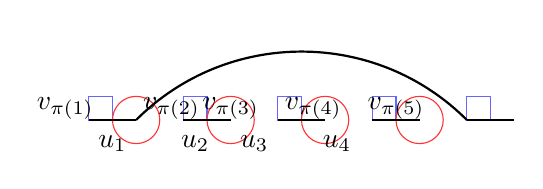
\begin{tikzpicture}[scale=1.5]
        % Vertices
        \filldraw[blue!60, fill=white] (0,0) rectangle (0.2,0.2) node[pos=0.5] {};
        \filldraw[red!80, fill=white] (0.4,0) circle (0.2);
        \filldraw[blue!60, fill=white] (0.8,0) rectangle (1,0.2) node[pos=0.5] {};
        \filldraw[red!80, fill=white] (1.2,0) circle (0.2);
        \filldraw[blue!60, fill=white] (1.6,0) rectangle (1.8,0.2) node[pos=0.5] {};
        \filldraw[red!80, fill=white] (2,0) circle (0.2);
        \filldraw[blue!60, fill=white] (2.4,0) rectangle (2.6,0.2) node[pos=0.5] {};
        \filldraw[red!80, fill=white] (2.8,0) circle (0.2);
        \filldraw[blue!60, fill=white] (3.2,0) rectangle (3.4,0.2) node[pos=0.5] {};
        
        % Edges
        \draw[thick, black] (0,0) -- (0.4,0);
        \draw[thick, black] (0.8,0) -- (1.2,0);
        \draw[thick, black] (1.6,0) -- (2,0);
        \draw[thick, black] (2.4,0) -- (2.8,0);
        \draw[thick, black] (3.2,0) -- (3.6,0);
        \draw[thick, black] (0.4,0) to[out=45,in=135] (3.2,0);
        
        % Labels
        \node at (-0.2, 0.1) {$v_{\pi(1)}$};
        \node at (0.2, -0.2) {$u_1$};
        \node at (0.7, 0.1) {$v_{\pi(2)}$};
        \node at (0.9, -0.2) {$u_2$};
        \node at (1.2, 0.1) {$v_{\pi(3)}$};
        \node at (1.4, -0.2) {$u_3$};
        \node at (1.9, 0.1) {$v_{\pi(4)}$};
        \node at (2.1, -0.2) {$u_4$};
        \node at (2.6, 0.1) {$v_{\pi(5)}$};
    \end{tikzpicture}
\caption{Illustration for the way in which the graph \( G' \) constructed in the proof of Case A of Lemma~\ref{lem:BE} can be embedded into the page of a book. The blue rectangles are B's vertices. In the example, \( j = 4 \).}
\end{figure}

\end{document}